\section{Exercise 1: Create a New Enemy}
    \begin{figure}[h]
        \centering
        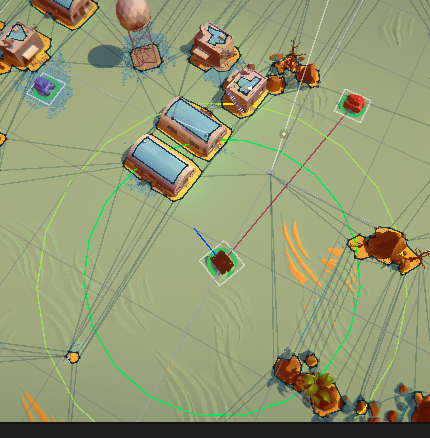
\includegraphics[width=0.5\textwidth]{imgs/tankai.png}
        \caption{The new enemy tank.}
        \label{fig:tankai}
    \end{figure}

\section{Exercise 2: Adjust the Camera}
    I added the new aiTank array to the previous existing targets array, then combined them.

    \begin{minted}{csharp}
        private void SetCameraTargets()
        {
            // Create a collection of transforms the same size as the number of tanks and AI tanks combined.
            Transform[] targets = new Transform[m_Tanks.Length + aiTanks.Length];


            for (int i = 0; i < m_Tanks.Length; i++)
            {
                // ... set it to the appropriate tank transform.
                targets[i] = m_Tanks[i].m_Instance.transform;
            }

            // Add AI tanks to the targets array.
            for (int i = 0; i < aiTanks.Length; i++)
            {
                targets[m_Tanks.Length + i] = aiTanks[i].m_Instance.transform;
            }

            m_CameraControl.m_Targets = targets;
        }
    \end{minted}

\section{Exercise 3: Point and Shoot}
    As seen in Figure \ref{fig:tankai}, the tank will follow the nearest player tank, and then get closer after the green circle touches the player. Then it will fire a shot every 2 seconds.
